\chapter{The Base Station}

Take a deep breath. We are about to put together out first major LCS hardware module. The previous chapters introduced the message format and protocols and the core library for implementing the event system as well as the running equipment based on the DCC signal standards. Next, we took a closer look on the major hardware building blocks and power module designs. Just like the LCS core library allows to build a node specific firmware on top, the hardware building blocks are the foundation to build the required hardware modules. We also looked at how one would go after designing the node firmware in general. So here is the first and most important hardware module putting it all together. The base station. Every layout needs to have some kind of a base station that acts as the central place for layout control and signal generation.

Looking at the market, there are plenty of so called base stations. They typically offer support for several standards and communication protocols, such as DCC, mfx, LocoNet, a Can Bus, a S88 sensor bus, and so on. Most base station also have the power module directly integrated. They support the configuration of locomotive and stationary decoders. In short, a one stop all round solution. Their price range is around few hundred Euros. With the advent of Arduino, Raspberry and other controllers there are numerous do it yourself solutions. Just to name one, the \texttt{DCC++} Arduino base station with a motor shield as a power unit, gets you a base station for well under hundred Euros. The excellent work of the JMRI community to provide a \texttt{DCC++} interface for configuration software and other utilities to use this inexpensive base station hardware. The DCC-EX group extended and stabilized the original \texttt{DCC++} work for a wider range of controllers but also with new capabilities. There are many such great projects. The appendix provides some links and pointers to this work.

\section{Key Requirements}

Our base station needs to deliver the following capabilities. At first it needs to be able to assemble the DCC packets and generate the respective DCC hardware signals. This work is split into the base station producing the signal content and the power section driving the hardware. Furthermore, the base station needs to provide a way to manage several locomotive sessions. For each active session the current state of the locomotive is maintained and the DCC packets are produced. When a new locomotive session is established, a dictionary of locomotives could be consulted about the particular locomotive to get the initial function settings, and so on.

A base station implementing locomotive session and track management should also implement a serial command interface for managing a session or sending commands to a locomotive. Although not really necessary, it is very beneficial for testing and debugging. But also, programming DCC decoders will need some form of getting the configuration data to the decoder. There are great openSource tools out there which make use of an ASCII interface to send their commands. An example is DecoderPro from the JMRI teams. It features among other protocols the \texttt{DCC++} ASCII interface to send and receive commands. Our base station will therefore implement the relevant \texttt{DCC++} commands.

All configuration settings, such as the number of concurrent sessions or the current consumption limit for a track, should be available as attributes on the node itself and ports. A track should be represented by a port, so there will be a port for controlling the MAIN track output, and a port for controlling the PROG tack output.

Finally, the firmware for the base station could also host LCS management functions, such as a configuration database or display data about layout operations. This is not per se a function of the base station, but as each layout needs to have a base station and perhaps display high level status data, it is a convenient place to put central functionality there as well. This subject will be discussed in another chapter, this chapter will focus on the core base station features.

\section{Base Station Hardware}

The base station is essentially based on a main controller board and a dual power module unit shown in previous chapters. We will use the PICO controller version and the dual H-Bridge building block. Add the RailCom detectors and stir the whole soup for a while. The extension connector of the base station would still export the I2C interface and the DCC signal produced by the base station. So, adding an I2C based extension board for display, switches, etc. is of course still possible. Here is the schematic for the base station. The individual building blocks should be familiar by now. The first page shows the main controller parts. Note that it needs fewer level shifters, as most of the signals are consumed internal to the board.

\begin{figure}[htbp]
    \centering
    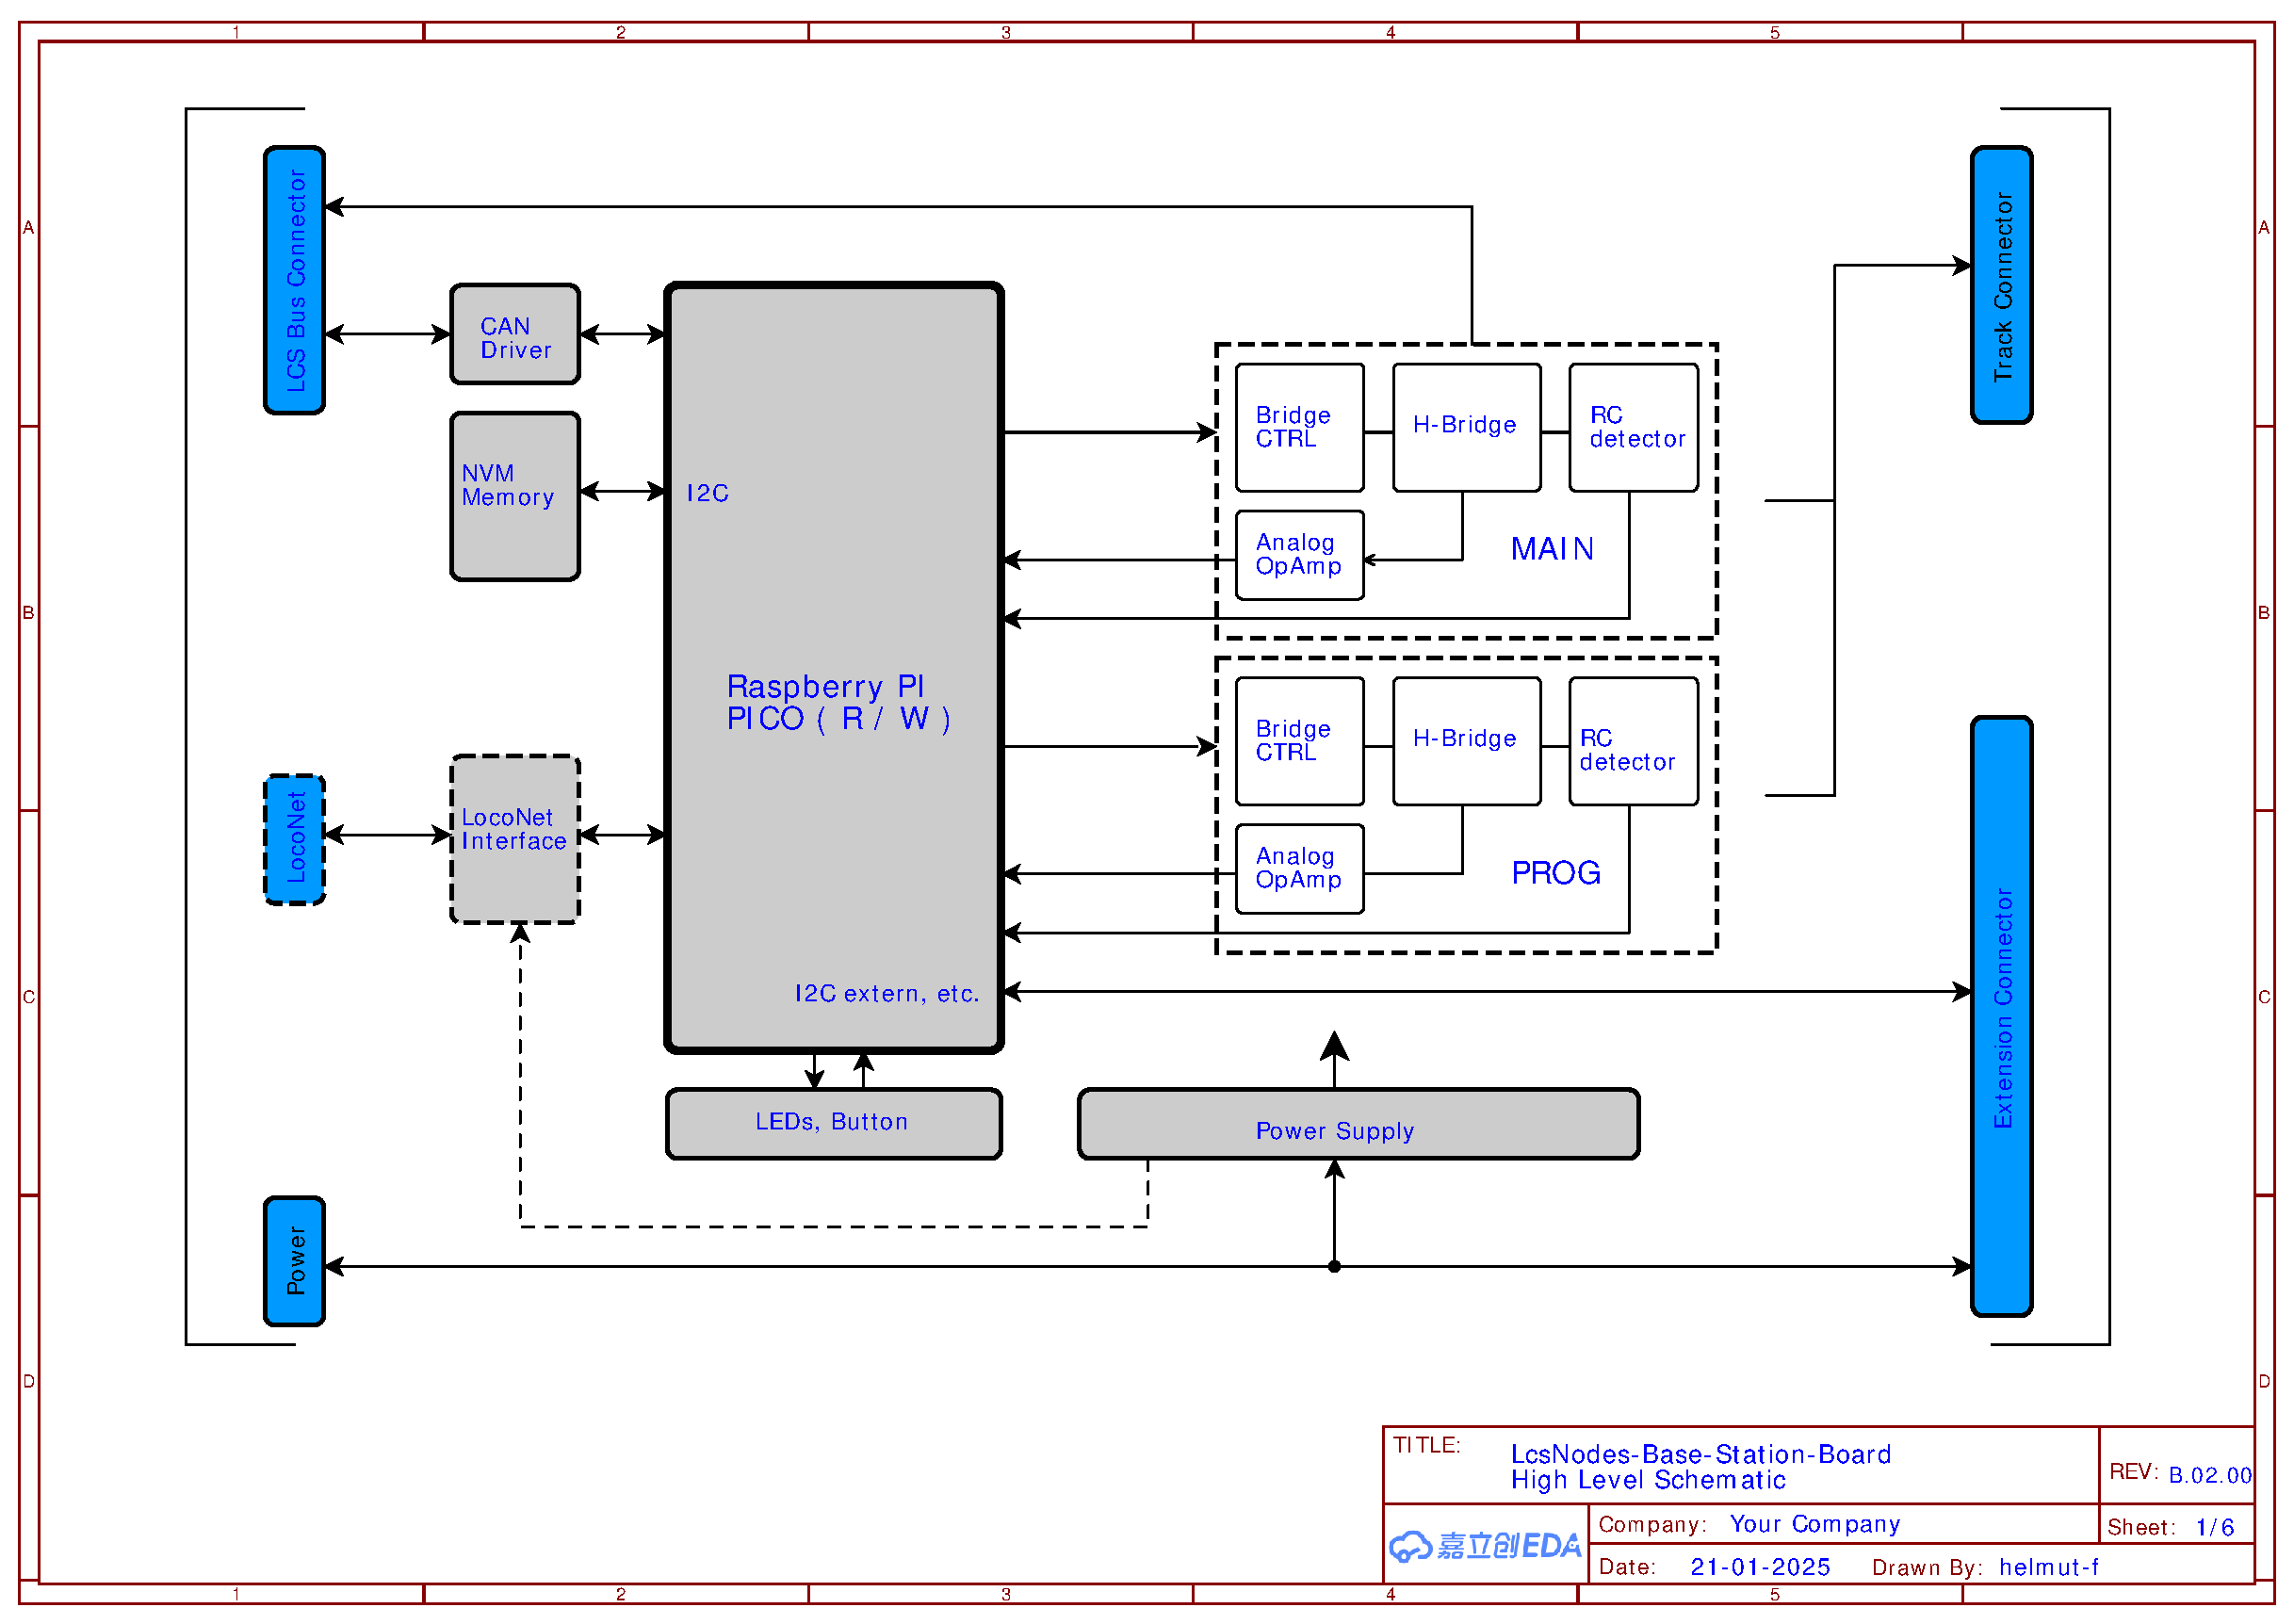
\includegraphics[page=1, width=0.9\textwidth]{./Schematics/Schematic_LcsNodes-Base-Station-Board.pdf}
    \caption{Block Diagram}
    %\label{fig:schematic}
\end{figure}
\FloatBarrier

\subsection{Base Station Main Controller}

The Raspberry PI Pico has enough capacity to implement the CAN bus protocol directly using one of the cores. As a result, only the line driver is necessary to implement the CAN bus interface. There are the level shifters for the I2C bus and a few other external signals. The Power supply needs to have a method to detect that there is an USB cable connected to the PICO and ensure that there is no conflict between the power sources. Like any LCS node, the controller needs a non-volatile memory. The base station hosts an I2C type NVM with up to 64Kbytes. The key reason for such a high capacity is that a base station might store a lot of data for each engine that it can manage.

\begin{figure}[htbp]
    \centering
    \includegraphics[page=2, width=0.9\textwidth]{./Schematics/Schematic_LcsNodes-Base-Station-Board.pdf}
    \caption{Main Controller}
    %\label{fig:schematic}
\end{figure}
\FloatBarrier

\subsection{Power Module}

The next part shows the power module. The power module exports the DCC signals via the external track power connectors and also as part of the LCS message bus connector connector. The track power extension connector is used by extension boards that directly use the H-Bridge output. A good example is an occupancy detector board which takes the DCC outputs and routes them to different sections, each equipped with a detectors for power consumption on the track. The power module unit features two identical channels. They are labelled "MAIN" and "PROG". Although the "PROG" channel would not need to deliver a high amperage, the dual H-Bridge is there anyway. And as said before, it would be nice to dynamically treat the PROG track as a type MAIN track too. 

\begin{figure}[htbp]
    \centering
    \includegraphics[page=3, width=0.8\textwidth]{./Schematics/Schematic_LcsNodes-Base-Station-Board.pdf}
    \caption{Power Module}
    %\label{fig:schematic}
\end{figure}
\FloatBarrier

\subsection{RailCom Detector}

Both channels also feature a RailCom detector. Refer to the base station firmware chapter on what we actually do with a RailCom detector. 

\begin{figure}[htbp]
    \centering
    \includegraphics[page=4, width=0.8\textwidth]{./Schematics/Schematic_LcsNodes-Base-Station-Board.pdf}
    \caption{RailCom Detector}
    %\label{fig:schematic}
\end{figure}
\FloatBarrier

\subsection{LocoNet Interface}

The base station will also offer an optional LocoNet interface. One day. LocoNet is very popular communication network for model railroads and there are a lot of devices such as Cab Handhelds that connect to the LocNet bus. Wouldn't it be nice to just connect these handhelds and alike via the LocoNet bus such that they can be used as well ? I guess it would. Right now, this is work in progress, but let's already reserve the the space on the board. Here is a first sketch of the interface.

\begin{figure}[htbp]
    \centering
    \includegraphics[page=5, width=0.8\textwidth]{./Schematics/Schematic_LcsNodes-Base-Station-Board.pdf}
    \caption{LocoNet Interface}
    %\label{fig:schematic}
\end{figure}
\FloatBarrier

\subsection{ Connectors and Power}

Finally, there are the connectors and the power supplies. While the LCS node runs with 5V as before, the LocoNet interface will offer 12V on its bus to connected devices. This part is also optional if LocNot is not implemented. In addition to the basic connectors that we have as part of the LCS node design, there are also two power connectors for the two tracks.

\begin{figure}[htbp]
    \centering
    \includegraphics[page=6, width=0.8\textwidth]{./Schematics/Schematic_LcsNodes-Base-Station-Board.pdf}
    \caption{Connectors and Power}
    %\label{fig:schematic}
\end{figure}
\FloatBarrier

\subsection{Base Station PCB}

The following picture shows the PCB for the monolithic base station. It is a 12cm by 10cm board, with the standard connectors in the usual place. As said, the LocoNet Interface is optional. 

\begin{tikzpicture}[scale=0.7, transform shape]

    \draw[help lines, gray!50, dashed] (0,0) grid( 16,8);
    \node at (8,4) {picture};

\end{tikzpicture}

Like the main controller, the monolithic base station board makes extensive use of SMD parts. While the previous boards have already been using passive SMD parts such as capacitors and resistors, this board also make use of SMD ICs. The exception is of course the Raspberry PI PICO board and the Dual H-Bridge IC L6205. The H-Bridge is a high power part and in case of a hardware problem it can easily be replaced as a DIP version.

\section{Base Station Firmware}

With the base station hardware in place, let's look at the firmware. First of all, the base station is just another LCS node and rests on the LCS runtime library. On top there is the locomotive session management, the DCC track power management, the DCC signal generation logic, and finally the RailCom communication interface. Being an LCS node, there are attributes and functions to control the base station through node and port items.

The base station is rather complex node. Especially the DCC signal generation requires the node to be very close to the controller chip capabilities. The individual parts will be described in the following sections. From an overall firmware perspective, the base station does its work in a functions that is called periodically from the LCS core library. The difference to other nodes is that the key work of producing the DCC signal is interrupt driven. There is a central timer that interrupts whenever the signals need to change their value is the central heartbeat of the node. Also, analog values are read with a start routine and an interrupt completer. The same is the case for the RailCom UART input. Everything that is part of the interrupt driven signal path will also just use interrupts for asynchronous execution. All else takes place outside the interrupt routines and is rather straightforward.

The base station module firmware is divided into a couple of key software modules. Let's start with locomotive session management.

\subsection{Locomotive Session Management}

The base station maintains a list of all active locomotives. Before controlling a locomotive or a consist, a session needs go be established. Once the session is place, LCS DCC commands such as set speed, direction and functions, are translated to the respective DCC packets according to standard. In addition, the standards require a periodic refresh of this data. The base station session management code will just run through the active sessions and issue the necessary DCC commands. Another key part of the base station functionality is the ability to configure a DCC decoder. Typically, the locomotive is put alone on special section of track. The configuration command will set CV values in the decoder. To configure a locomotive on the programming track, no session is actually required. As programming an engine is in the end also just a matter of sending DCC packets, the functionality is part of the session management object.

Locomotive session management is closely interacting with the DCC track management object. The primary task is to put the DCC packets generated out on the track. Also, for programming a DCC decoder, the CV value configuration requires the detection of a change in track power current consumption. The design separates the signal generation from session management. The key linkage is the submission of a packet. As we will see in the track management section, the signal generation is a typical timer interrupt driven game. Whenever a new bit should be sent to the tracks, the interrupt handler sets the signal lines which drive the power module and sets the timer values when to become active next. There are designs out there that let the interrupt handler also directly interact with the session table to get the next bit from the current packet. Our route is a clear separation of both parts. All locomotive session management does is to produce the packets and submit them. Putting bits out from a DCC packet is the duty of the companion module DCC track management.

As the layout and the number of running engines grows, the DCC bus may reach its limits. There are roughly about 100 DCC messages that can be sent to the track per second. Using the DCC track just for running engines already helps greatly. But if the base station has to deal with hundreds of locomotives, a priority management of what packets go in which order is perhaps required. The simple approach of the locomotive session just sending out the DCC command needs to be replaced with a more clever refresh scheme. For example, deceleration commands need to be given a higher priority than acceleration commands. It is more important to stop an engine than to accelerate one. The function refresh option needs to interleave speed and function group refresh commands to guarantee that the speed command is repeated often. A loco with a speed of zero, has rather low priority, the engine is not considered active. The DCC standards require that each active decoder, i.e. a decoder with a loco that has a non-zero speed, is refreshed at least every 2.5 seconds.

In general, base stations are required to send a valid DCC packet every 30 milliseconds to indicate that the DCC protocol is still active. Further more, there should be a time gap of at least 5 milliseconds between two packets addressing the same decoder. The base station itself is required to send every 5 seconds what its capabilities are. For example, the base station can broadcast that it supports 128-step speed setting. There are also attributes for stationary decoders as well. Finally, the base station broadcasts a "layout" time. This can be used by all decoders to simulate timing aspects of their features.

// ??? \textbf{note} update the following paragraph when the session management refresh work is implemented... we need a more global approach to periodic work in the code ...

Right now, the scheme is simple. A DCC management LCS message directly results in the DCC command sent to the track. The refresh function just advances through the session map and emits a DCC refresh packet for each active session. More experience with a really large layout is needed before changing this simple approach.

\subsection{Base Station Global Functions}

In addition to locomotive session management and the DCC track management, a base station is also responsible for global data such as the system data and time. Each decoder can make use of this "layout" time. The base station is required to send out this information periodically. Furthermore, the base station needs to broadcast what global capabilities and configuration options are available. For example, the base station will communicate which standards are supported, whether it supports a 128-step speed setting or not, wether  programming on the main track is enabled and on on. The base station is required to send this kind of information every 5 seconds.

\subsection{Locomotive Session Management Attributes and Functions}

Locomotive session management presents itself through a set of node attributes and functions.

// \textbf{note} fill in what we can access through the node/port interfaces

%|Item|Arguments|Purpose|
%|:--|:--|:--|
%| ... | ... | ... |

\subsection{DCC Track management}

Here we are with a stream of DCC packets send by the locomotive session management. To get the DCC packet actually onto the track, DCC track management component has two key functions. There is the signal generation part and the track power management part.

\subsection{DCC Track Signal Management}

The base station produces for the main track and programming track the DCC signal. To recap, the DCC ONE bit is a square wave signal with a period of 58 microseconds, the DCC ZERO bit a square wave signal with a period of 116 microseconds. A signal generation logic could thus think in "ticks" of 58 microseconds. However, when implementing RailCom support a cutout period needs to be added. This period starts with a 29us ONE followed by the cutout period itself, followed by 29us ZERO to complete the cutout. Luckily, 29 is two times 58. A DCC "ONE" is therefore two ticks of 29us "+" follow by two ticks of "-" on the signal generation lines.

// ??? \textbf{note} repeat the DCC picture here ? NO. make a new picture... ( signal, cut, Z-blackout, etc ).

The software implementation used in the base station consists of a track signal state machine and one timer that can be scheduled to interrupt in multiple of 29 microseconds. Whenever the interrupt happens  the interrupt logic first sets the new signal levels and then computes the next interrupt timer value in ticks. Since we have two tracks and control both state machines with one timer, the next time to interrupt is the smaller number of ticks for the two tracks. For example, if one track is scheduled to change the signal level in 2 ticks, the other track in 4 ticks, the interrupt timer is set to interrupt again in 2 ticks. At that time, the track that wants to be interrupt in 4 ticks, does nothing but to decrement the tick interrupt count to 2.

Running both state machines with one timer also requires that we split the work of the state machine in two parts. First, each state machine takes care of setting the hardware signal levels. It is essential that both tracks get their signal marching orders as soon as possible to maintain an accurate DCC signal timing. But there is more work to do. Each track state machine can therefore might request some further work. For example, we need to get the next DCC packet bit and if all bits are processed the next DCC packet lined up for transmission. Once both state machines have set their signal levels, the follow up actions are processed.

In addition to getting the next bit or packet, there is the requirement to measure the actual power consumption. Power consumption measurement is essentially measuring a voltage using the ADC hardware the controller. The AtMega does have multiple ADC channels, but can use only one channel at a time. The DCC track signal state machine will thus in a conflict prefer to measure the main track. There are a couple of ways where this measurement can be done. The easiest is to just sample the current consumption in sync with the DCC signal and store it away. The LCS base station power module does this during a DCC ZERO bit in the middle of the first half wave period. The value is stored in the DCC track object, overwritten each time there is a measurement. Depending on the packets content a few hundred sample will be taken per second.

While this approach will work fairly reasonable, there is a hidden challenge though. The measurement will sample what the current consumption is. And this consumption depends on the actual power drawn by the decoder. Since decoders typically drive the engine motor with a PWM signal, it matters when the measurement is taken. With a decoder with a low PWM frequency there is a good chance to measure during the "off" period of the PWN signal. It will be therefore be important to measure very often and compute a mean value, for example a Root Mean Square" value, across a significant sample of measurements. However, we need to make sure that the controller is not overwhelmed with all the processing that needs to be done. Our approach is to measure quite often and store the digital values. Short circuit detection and also a simple high water mark computation can be be done with little overhead. Only when an RMS value is needed, the square root of the sum of squares of our samples is computed and converted to milliAmps. Note that that the RMS computation is done using 16-bit unsigned integers. This is little less precise compared to a floating point value computation, but the performance gain from using integer math justify this moderate imprecision.

\subsection{Track Signal management using Raspberry Pi Picos features}

The Raspberry PI Pico has a very powerful feature, which are the PIO state machines. Rather than offering various IO interfaces and protocols in dedicated silicon blocks, the PIO state  machines are programmable IO controllers. One idea is to just implement the DCC output though a PIO program. A tempting project.

However, right now the SW state machine described before will just work fine and do the job for both controller families. May some time later.

\subsection{Track Power Management}

In addition to the signal generation state machine, there is a track power state machine. This state machine runs periodically and checks for power overload. When the power consumption exceeds the configured limit, the track is shut down. After a short period of time restart is attempted. If the restart leads again to a power overload and this happens for several attempts, the track is shut down permanently. Manual action is necessary.

For the programming track, the power consumption measurement plays another very important role. A decoder to be programmed using the CV value access DCC packets can only answer with a temporary raise of its own power consumption. The standards defines a raised current consumption by 60mA for 5 to 7 milliseconds as a positive acknowledgement. Accessing a CV variable consists of sending a sequence of DCC packets. First there is a set of RESET packets, followed by the CV commands, followed by RESET packets. During the first RESET packets, the power consumption is measured and a baseline for a "normal" decoder power consumption is established. When the decoder later answers to a request by raising its power consumption this baseline is used to detect it.

With RailCom implemented, a decoder can also be configured using the programming on the main (POM) DCC commands with status and data reply via RailCom datagrams. More on this in a later section.

\subsection{Base Station Dictionary}

Another software component typically found in base stations is a dictionary. For each locomotive there is a dictionary entry that describes this locomotive. When a session for that locomotive is allocated, this entry is consulted and initial values for speed, direction and other functions are set.

// ??? \textbf{note} we just do locos. How to put data in and read data out ?

%|Item|Arguments|Purpose|
%|:--|:--|:--|
%| ... | ... | ... |

\subsection{DCC Track Management Attributes and Functions}

// \textbf{note} fill in what we can access through the node/port interfaces

%|Item|Arguments|Purpose|
%|:--|:--|:--|
%| ... | ... | ... |

\subsection{RailCom Support}

For RailCom support the power module is directed to short circuit the track for a defined period before working on the next packet. The DCC decoder in the locomotive will detect this short circuit or cutout period and send a RailCom datagram. During this period the controller attempts to read in the datagram bytes from the serial I/O input line. Both analog measurement as well as serial I/O reading for RailCom are implemented as a setup the request routine followed by an interrupt routine that processes the results in as little as possible time. After all, our key priority is the correct DCC signal timing.

\subsection{RailCom Support Attributes and Functions}

// \textbf{note} fill in what we can access through the node/port interfaces
// \textbf{note} channel one will always fill a port variable with what ever the loco ID currently is. Can be read by all nodes...
// \textbf{note} channel two will essentially invoke a callback to deal with the data received on a POM/XPOM request.


%|Item|Arguments|Purpose|
%|:--|:--|:--|
%| ... | ... | ... |

\subsection{LocoNet Support}

// ??? \textbf{note} under investigation. We would need a library to send and receive the locoNet messages. We also would need a higher level piece to "understand" these messages and translate them to LCS messages. From a HW perspective, perhaps one PIO block of the PICO is needed to implement a UART, as the two UARTS are used for RailCom already... in other words a bigger research project :-).

\section{Base Station Serial Commands}

In addition to the LCS core library serial commands available to any node, the base station implements a serial command interface which accepts a subset of the \texttt{DCC++} / DCC-EX commands. As a short introduction, \texttt{DCC++} was an implementation of a DCC base station using an Arduino Uno and a motor shield. For a very small budget and with little effort, the world of DCC opened up to everyone. Part of the \texttt{DCC++} system is an ASCII interface to send commends to the base station. Not only is this command line feature useful for debugging the base station code, it is really valuable when interfacing to tools such as Decoder Pro provided by the JMRI organization, which implemented an ACCI interface to \texttt{DCC++}. The command listed in the table below are an accurate implementation of the original DCC++ commands. In addition some commands have been added.

\begin{longtable}{@{}|l|p{0.2\linewidth}p{0.6\linewidth}@{}}
    \caption{Table Caption} \\
    \toprule
    \textbf{Command} & \textbf{Reply} & \textbf{Operation}\\
    \midrule
    \endfirsthead
    \toprule
    \textbf{Command} & \textbf{Reply} & \textbf{Operation}\\
    \midrule
    \endhead
    \midrule
    \multicolumn{2}{r}{\textit{Continued on next page}} \\
    \midrule
    \endfoot
    \bottomrule
    \endlastfoot
    Row1 & \textbf{Row1} & Text1 \\
    \midrule
    Row2 & \textbf{Row2} & Text2 \\
\end{longtable}

| O | cabId | | allocate a session for the cab|

| K | sessionId | | release a session |

| t | sessionId cabId speed direction>| | set cab speed / direction|

| f | cabId funcId val | | set cab function value, function group DCC format |

| v | sessionId funcId val| | set cab function value, individual |

| R | cvId callbacknum callbacksub | | read CV byte on the programming track |

| W | cvId val callbacknum callbacksub | | write CV byte on the programming track |

| B | cvId bitPos bitVal callbacknum callbacksub | | write CV bit on the programming track |

| b | cabId cvId bitPos bitVal | | write CV bit on the programming track |

| w | cabId cvId val | | write CV byte on the operations track |

| M | sessionId byte1 byte2 [ byte3 ... byte10 ] | | send DCC packet on operations track |

| P | sessionId byte1 byte2 [ byte3 ... byte10 ] | | send DCC packet on programming track |

| X | | | emergency stop all |

| 0 | | | turn operations and programming track power off |

| 1 | | | turn operations and programming track power on |

| 2 | | | turn operations power on |

| 3 | | | turn programming track power on |

| a | [ opt ] | | list current consumption, where opt=0 -> MAIN (default ), opt=1 -> PROG, opt=2 -> both |

| C | [ option ] | | set options for the track. 0 -> set service track in operations mode, 1 - > set service track in service mode, 2 -> enable RailCom, 3 -> disable RailCom |
| s | [ level ] | | list status at detail level, default is summary. 0 -> summary, 1 -> configuration,  2 -> session map |

| S | | | list base station configuration |

| L | | | list base station session table |

| D | | | enter diagnostics mode - need to restart later! |

| ? | | | list this help |

























\section{Summary}

The base station, no matter how it is implemented, is a key component in any digital layout. It is primarily responsible for the locomotive session management and track signal generation. There could be designs where the base station is a device in a nice housing with a display, switches and so on. Other designs just put the LCS node somewhere on the layout. All these options will work just fine. And just like any other LCS node, the base station firmware offers through node and port attributes status and control functions.

The base station was also the first major LCS node with a considerable amount of hardware and software and thus went to several iterations and a considerable amount of learning curves. The very first version started with an Arduino Mega and Motor driver breakout board. The software was the original DCC++ software. The next versions actually were just a refactoring effort and work on the software. I learned a great deal on how all this works. The next base station version was a single board with all possible interfaces on an experimental PCB. It already featured CAN BUS, dual H-Bridges, and a controller, the Atmega 1284. This board served a long time for software development and further experiments. The next version of the base station was built with a main controller PCB described in the earlier chapters and a dual power unit, that also featured the RailCom detector. And again further software refactoring, refinement and learning. Finally, after a switch to the Raspberry Pi Pico controller, first on breadboard  then on PCBs, the base station shown in this chapter is the current version. The lessons learned proved to be very valuable for the overall concept development and hardware design. And in addition, there was a great deal of reading on chip specifications and, very importantly, the DCC standards. The appendix contains a list of material and web links. I highly recommend to read the electrical and DCC related standards published by the RailCommunity organization.


// ??? \textbf{note} wrap it up ..

Just like any other LCS node, the base station firmware offers through node and port attributes status and control functions. However, there is only one on the layout.

The base station was also the first major LCS node with a considerable amount of hardware and software. Initial work started with the main controller and power module extension board based on the Atmega processor family. From there, a monolithic version using the Raspberry PI PICO was developed and that is the latest base station offering.

What is next ?. Well, we have a base station and with the simple command interface it is possible to open a loco session and control that engine. But this command interface is rather for software development and debugging. What we really want is of course a handheld of some form with buttons and levers. So, before building boosters, block controller and extension boards and firmware, the next chapters will develop a handheld. 

